\documentclass[11pt,oneside,a4paper]{article}


% Packages to use
\usepackage{graphicx}
\usepackage{hyperref}
\usepackage{amsmath}
\usepackage{amssymb}
\usepackage{amstext}
\usepackage{amsthm}
\usepackage{palatino}
\usepackage[a4paper]{geometry}
\usepackage[dvips]{color}
\usepackage[toc,page]{appendix}
\usepackage{sectsty}


\theoremstyle{definition}
\newtheorem{definition}{Definition}
\newtheorem{example}{Example}


\title{Visualization of $\beta$-reduction-graphs in the lambda calculus}
\author{Niels Bjørn Bugge Grathwohl & Jens Duelund Pallesen}
\date{\large \today}


%  New color
\definecolor{sectionColor}{RGB}{65,117,78}


% Color & size for sections
\sectionfont{\huge\color{sectionColor} }
\subsectionfont{\large\color{sectionColor} }


% Margins
\geometry{top=2.0cm, bottom=2.0cm, left=2.0cm, right=2.0cm}


% Custom commands
\newcommand{\Z}{\mathbb{Z}}
\newcommand{\R}{\mathbb{R}}
\newcommand{\N}{\mathbb{N}}
\newcommand{\lam}[2]{\lambda#1.#2}
\newcommand{\BETA}{\boldsymbol\beta}
\newcommand{\barrow}{\rightarrow_\beta}
\newcommand{\Barrow}{\barrow^*}
\newcommand{\I}{\textsf{\textbf{I}}}


%%%%%%%%%%%%%%%%%%%%%%%%%%%%%%%%%%%%%%%%%%%%%%%%%%
\begin{document}
%%%%%%%%%%%%%%%%%%%%%%%%%%%%%%%%%%%%%%%%%%%%%%%%%%

% Title page
% %!TEX root = rapport.tex

\begin{titlepage}
 
\begin{center}
 
 
% Front page image
\includegraphics[scale=0.75]{titleLogo.jpg}\\[4.0cm]
 
 
% Title
\textcolor{newblue}{{\huge \bfseries Visualization of $\beta$-reduction-graphs in the lambda calculus}\\[2.0cm]}
% Author and supervisor
\begin{minipage}{0.4\textwidth}
\begin{flushleft} \large
\emph{Author:}\\
Niels Bjørn Bugge Grathwohl\\
Jens Duelund Pallesen
\end{flushleft}
\end{minipage}
\begin{minipage}{0.4\textwidth}
\begin{flushright} \large
\emph{Supervisor:} \\
Jakob Grue Simmonsen
\end{flushright}
\end{minipage}
 
\vfill
 
% Bottom of the page
{\large \today}
 
\end{center}
 
\end{titlepage}
% \newpage

% Abstract
%!TEX root = rapport.tex

\begin{abstract}

\textbf{Background} This is a project in how to visualize reduction graphs in
the lambda calculus. It is a part of the master education in Computer Science
at the University of Copenhagen. Our focus in this project is to implement a
piece of software in Python, that can visualize reduction graphs in a
``pretty'' and informative way. The target group for the project is
theoretical computer scientists with an interest in the lambda calculus. We
will, besides Python implementation, work with both general lambda calculus
theory and visualization / graph theory.

\textbf{Results} Our results are...

\textbf{Conclusion} The conclusion is...

\end{abstract}
\newpage

% Table of content
\tableofcontents
\listoftables
\listoffigures
\newpage

% Chapters
%!TEX root = rapport.tex

\section{Preliminaries: Basic Lambda Calculus}

The untyped lambda calculus was introduced in 1936 by Alonzo Church
[reference] as part of the search for a solid foundation for mathematics. It is
heavily intertwined with the notion of a ``function'', in the sense that logic
and mathematics is represented with only functions and untyped variables that
can be either free or bound.


% alt er funktioner
% eksempler

As a very informal example, here is a function that doubles an integer:
\begin{equation*}
	(\lam{x}{x+x})2=4
\end{equation*}
This example shows a bound variable, $x$, and an implicit \emph{reduction} step. The variable $x$
is said to be bound because the lambda function uses it as an argument. Contrast this to
\begin{equation*}
	(\lam{x}{x+y})2=2+y.
\end{equation*}
Here, $y$ is a free variable that hasn't got any values assigned to it yet. It can
take any value, hence it's called ``free''. In this second example there was
another reduction step. A reduction step can be regarded as a rewriting action
on the string representing the lambda expression. Yet more informally, one can 
think of it as ``substituting in'' the values. In the examples above this amounts to
replacing $x$ with the number 2. 

% definition af syntax

The lambda calculus consists of \emph{lambda expressions} and variables with a
recursively defined syntax. The set of all lambda expressions is denoted $\Lambda$:
\begin{align*}
	x \text{ is a variable} &=> x\in\Lambda \\
	x \text{ is a variable and } M\in\Lambda &=> (\lam{x}{M})\in\Lambda \\
	M, N\in\Lambda &=> (M N)\in\Lambda
\end{align*}
For brevity, it's convention to leave out the outermost parentheses.
Expressions are evaulated left-to-right, so $M N P = (M N) P$, and function
bodies extend as far as possible; $\lam{x}{M N}=\lam{x}{(M
N)}\neq(\lam{x}{M})N$.

% frie variable
As already indicated, the variabled in a lambda expression can be split on two groups;
the free and the bound variables. The function $FV$ takes returns for any
lambda expression the set of free variables:
\begin{align*}
	FV(x)&={x} \\
	FV(\lam{x}{M})&= FV(M) \backslash {x} \\
	FV((M N)) &= FV(M) \cup FV(N)
\end{align*}

% definition af alfakonvertering
% eksempel
% definition af betareduktion
% eksempel!
% definition af reduktionsgraf
% eksempel(?)


% Syntax

% Alpha-conversion

% Beta-reduction
%!TEX root = rapport.tex

% \textcolor{navyblue}{\section{Existing visualizations in lambda theory}}
\textcolor{newblue}{\section{Evaluation of existing visualizations in lambda theory}}
According to our research, there does not exist anything exactly similar to our theses exist. There does on the other hand exist visualizations of other lambda-related areas. In this section we will discuss these.

There are numerous examples where a lambda term or a given reduction for a lambda term has been visualized. We have in in just a few hours of research found XX examples of this [See appendix A].

What differentiates these examples from this project is mainly two things:
\begin{itemize}
	\item It is currently not possible to get a complete overview of all the reductions and thereby get an understanding of how the lambda term evaluate over time.
	\item Secondly, non existing visualizations has been capable of doing it beautifully.
\end{itemize}

We will in the rest of this chapter describe three of these examples, which we have selected to be the most interesting.

\subsection{Alligator Eggs -  A Puzzle Game by Bret Victor}

\begin{figure}
	\begin{center}
   		
\includegraphics[scale=0.5]{images/AlligatorEggs.png}
		\caption{Alligator Eggs -  A Puzzle Game}
	\end{center}
\end{figure}

The ``Alligator Eggs -  A Puzzle Game'' \cite{Alligator} is a fun and children-like way of visualizing the computation of a lambda term. It self and is not directly related to our thesis concerning evaluation of the $\beta$-reduction-graphs of the lambda term.\\

The theory in this game is based on the untyped lambda calculus. The game rules is defined according to the following:
\begin{enumerate}
	\item A hungry alligator is a lambda abstraction
	\item An old alligator is parentheses
	\item Eggs are variables
	\item The eating rule corresponds to a $\beta$-reduction
	\item The color rule corresponds to alpha-conversion
	\item The old age rule says that if a pair of parentheses contains a single term, the parentheses can be removed\\\\
\end{enumerate}

In the example below we the eating rule in use. The green alligator will whatever is in front of it. In this case it will eat the yellow alligator and its yellow egg. After the green alligator has eaten the yellow alligator and egg it will die and its egg will hatch into what it has eaten. The miracle of life, as the author calls it. This little episode is, as stated in the definition, corresponding to a $\beta$-reduction. 

\begin{figure}
	\begin{center}
		
\includegraphics[scale=0.5]{images/alligatorEat.png}
		\caption{A reduction visualized as an alligator eating}	
	\end{center}
\end{figure}

The ``Alligator Eggs -  A Puzzle Game'' does not deal with the same lambda theory as we do in our theses. It does although deal with being visually attractive.

The ``Alligator Eggs -  A Puzzle Game'' has also been implemented in a tool using Java. \cite{AlligatorTool}


\subsection{Lambda Animator by Mike Thyer}
The ``Lambda Animator'' is a representation of lambda expressions in tree form. It is implemented in Java and available online via a Java Applet.

\begin{figure}
	\begin{center}
		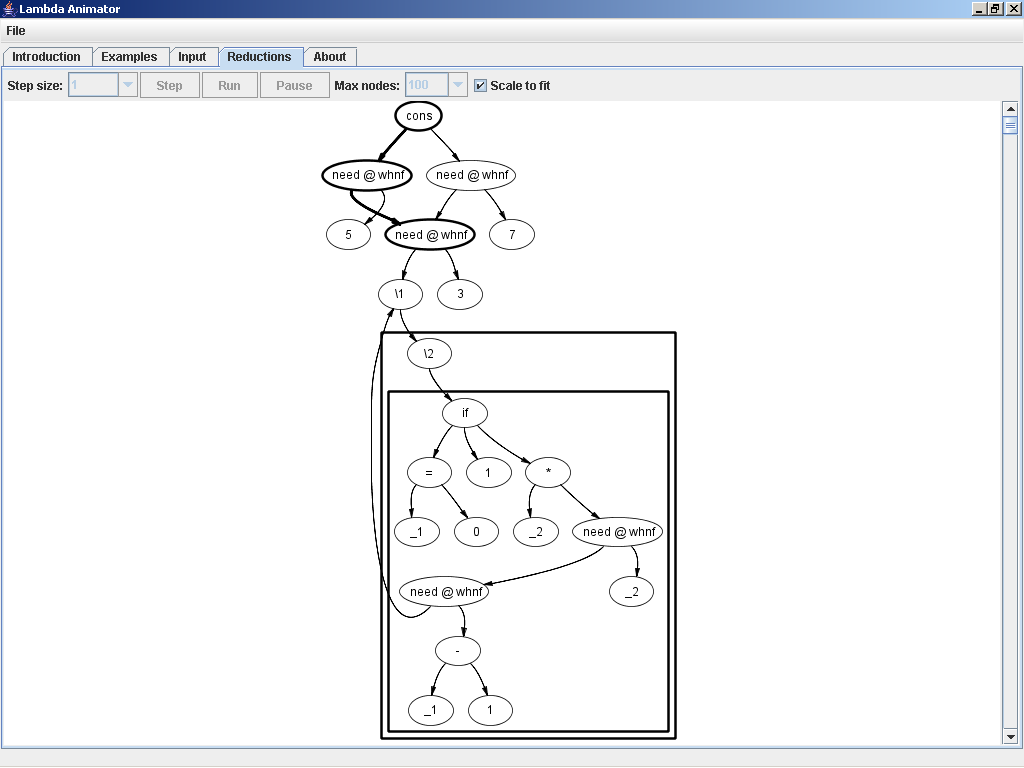
\includegraphics[scale=0.35]{images/lambdaAnimator.png}
		\caption{Screenshot of the Lambda Annimator tool}	
	\end{center}
\end{figure}

The animator does not seem very smooth and does not produce graphs that are neither pretty or especially informative. It uses extremely simple graphics and does not fulfill our ``pretty'' criteria. The implementation in Java (Applet) is although advantageous in terms of easy access to the tool.

% Appendices
\appendix
\appendixpage
\section{Examples of visualized lambda}
%!TEX root = rapport.tex

\chapter{Next appendix}\label{app:b}
%!TEX root = rapport.tex

\chapter{And the following}\label{app:c}

% Bibliography
\newpage
\bibliographystyle{plain}
\bibliography{bibliography}

%%%%%%%%%%%%%%%%%%%%%%%%%%%%%%%%%%%%%%%%%%%%%%%%%%
\end{document}
%%%%%%%%%%%%%%%%%%%%%%%%%%%%%%%%%%%%%%%%%%%%%%%%%%
